% Name: Polar coordinates of a point
% Description: The point P = (r, θ) = (3, π/3) on a polar grid: its distance r from the pole O and its angle θ from the polar axis.
% Tags: polar coordinates, polar grid, angle, trigonometry

\usetikzlibrary{arrows.meta}

\begin{tikzpicture}[>={Stealth}, every node/.style={font=\small}, scale=0.85]
  \foreach \r in {1,...,4} \draw[gray!30] (0,0) circle (\r);
  \foreach \a in {0,30,...,330} \draw[gray!30] (0,0) -- (\a:4);
  \foreach \a/\t in {90/{\frac{\pi}{2}}, 180/{\pi}, 270/{\frac{3\pi}{2}}} \node[gray!70!black] at (\a:4.45) {$\t$};
  \foreach \r in {1,...,4} \node[below, gray!70!black, font=\scriptsize] at (\r,0) {$\r$};
  \draw[->] (0,0) -- (4.6,0) node[right] {polar axis};
  \fill[orange!25] (0,0) -- (1.1,0) arc[start angle=0, end angle=60, radius=1.1] -- cycle;
  \draw[orange!85!black] (1.1,0) arc[start angle=0, end angle=60, radius=1.1];
  \node at (30:1.45) {$\theta$};
  \draw[->, very thick, blue!70!black] (0,0) -- node[above left] {$r$} (60:3);
  \fill (0,0) circle (1.5pt) node[below left] {$O$};
  \fill[blue!70!black] (60:3) circle (2pt) node[above right] {$P\,(3, \tfrac{\pi}{3})$};
\end{tikzpicture}
